\usetikzlibrary{decorations.markings}
\tikzset{
  strand/.style={semithick}, 
  dstrand/.style={dotted}, 
  rdstrand/.style={semithick,dash pattern=on 0.7 off 1pt, color=red},  
  oriented/.style={postaction={decorate},
                   decoration={markings, mark=at position 0.85 with {\arrow{>}}}} 
}



\newcommand{\undercross}[2]{
  \vcenter{\hbox{\begin{tikzpicture}[scale=0.6]
    \draw[#1,oriented] (-0.6,-0.6) -- (0.6,0.6);
    \draw[white,line width=5pt] (0.6,-0.6) -- (-0.6,0.6); 
    \draw[#2,oriented] (0.6,-0.6) -- (-0.6,0.6);
  \end{tikzpicture}}}
}


\newcommand{\unundercross}[2]{
  \vcenter{\hbox{\begin{tikzpicture}[scale=0.6]
    \draw[#1,oriented] (-0.6,-0.6) -- (0.6,0.6);
    \draw[white,line width=5pt] (0.6,-0.6) -- (-0.6,0.6); 
    \draw[#2,oriented] (0.6,-0.6) -- (-0.6,0.6);
  \end{tikzpicture}}}
}
\newcommand{\overcross}[2]{
  \vcenter{\hbox{\begin{tikzpicture}[scale=0.6]
    \draw[#2,oriented] (0.6,-0.6) -- (-0.6,0.6); 
    \draw[white,line width=5pt] (-0.6,-0.6) -- (0.6,0.6); 
    \draw[#1,oriented] (-0.6,-0.6) -- (0.6,0.6); 
  \end{tikzpicture}}}
}


\newcommand{\parallelstrands}[2]{
  \vcenter{\hbox{\begin{tikzpicture}[scale=0.6]
    \draw[#1,oriented] (-0.4,-0.6) -- (-0.4,0.6);
    \draw[#2,oriented] (0.4,-0.6) -- (0.4,0.6);
  \end{tikzpicture}}}
}


\newcommand{\singlestrand}[1]{
  \vcenter{\hbox{\begin{tikzpicture}[scale=0.6]
    \draw[#1,oriented] (0,-0.6) -- (0,0.6);
  \end{tikzpicture}}}
}


\newcommand{\loopstrand}[1]{
  \vcenter{\hbox{\begin{tikzpicture}[scale=0.6,xscale=-1]
    \draw[#1,oriented]
      (0,-0.6) .. controls +(0,0.5) and +(-0.4,0) .. (0.3,0)
                .. controls +(0.4,0) and +(0,0.5) .. (0,0.6);
  \end{tikzpicture}}}
}
\newcommand{\loopstrandJ}[1]{
  \vcenter{\hbox{\begin{tikzpicture}[scale=0.6,,xscale=-1]
    \coordinate (C) at (-0.1,0);
    \coordinate (X) at (-0.1,-0.6);
    \coordinate (Y) at (-0.1,0.6);
    \coordinate (A0) at (0.1,0.1);
    \coordinate (A1) at (0.1,-0.3);
    \coordinate (B) at (0.3,-0.1);
    \draw[#1] (A1) [out=180,in=-80] to (C);
    \draw[#1,oriented] (C) [out=100,in=-90] to (Y);
    \draw[white,line width=4.5pt] (X) [out=90,in=-100] to (C);
    \draw[white,line width=4.5pt] (C) [out=80,in=90] to (B);
    \draw[white,line width=4.5pt] (B) [out=-90,in=0] to (A1);
    \draw[#1] (X) [out=90,in=-100] to (C);
    \draw[#1] (C) [out=80,in=180] to (A0);
    \draw[#1] (A0) [out=0,in=90] to (B);
    \draw[#1] (B) [out=-90,in=0] to (A1);
  \end{tikzpicture}}}
}



\newcommand{\circlestrand}[2]{
  \vcenter{\hbox{\begin{tikzpicture}[scale=0.6]
    \ifthenelse{\equal{#2}{ccw}}{
      \draw[#1,oriented] (0,0) circle (0.5);
    }{
      \draw[#1,oriented] (0.5,0) arc[start angle=0,end angle=-360,radius=0.5];
    }
  \end{tikzpicture}}}
}


\newcommand{\Nvertex}[1]{
  \vcenter{\hbox{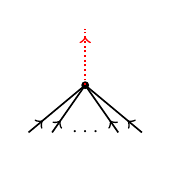
\begin{tikzpicture}[scale=0.6]
    \tikzset{lowarrow/.style={semithick, postaction={decorate},
                               decoration={markings, mark=at position 0.25 with {\arrow{>}}}}}

    \draw[strand,lowarrow] (-1.2,-1.2) -- (0,-0.2);
    \draw[strand,lowarrow] (-0.7,-1.2) -- (0,-0.2);

    \node at (0,-1.2) {\scriptsize $\cdots$};

    \draw[strand,lowarrow] (0.7,-1.2) -- (0,-0.2);
    \draw[strand,lowarrow] (1.2,-1.2) -- (0,-0.2);

    \filldraw (0,-0.2) circle (2pt);

    \draw[rdstrand,oriented] (0,-0.2) -- (0,1.0);
  \end{tikzpicture}}}
}

\newcommand{\dualNvertex}[1]{
  \vcenter{\hbox{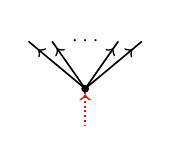
\begin{tikzpicture}[scale=0.6]
    \tikzset{lowarrow/.style={semithick, postaction={decorate},
                               decoration={markings, mark=at position 0.25 with {\arrow{<}}}}}

    \draw[rdstrand,oriented] (0,-1.0) -- (0,-0.2);

    \filldraw (0,-0.2) circle (2pt);

    \draw[strand,lowarrow] (-1.2,0.8) -- (0,-0.2);
    \draw[strand,lowarrow] (-0.7,0.8) -- (0,-0.2);

    \node at (0,0.8) {\scriptsize $\cdots$};

    \draw[strand,lowarrow] (0.7,0.8) -- (0,-0.2);
    \draw[strand,lowarrow] (1.2,0.8) -- (0,-0.2);
  \end{tikzpicture}}}
}

\newcommand{\NtoNvertex}[1]{
  \vcenter{\hbox{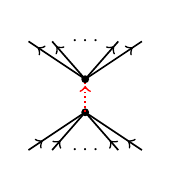
\begin{tikzpicture}[scale=0.6]
    \tikzset{
      lowarrow/.style={semithick,postaction={decorate},
                        decoration={markings, mark=at position 0.25 with {\arrow{>}}}},
      dashedarrow/.style={semithick,postaction={decorate},
                           decoration={markings, mark=at position 0.8 with {\arrow{>}}}},
      outarrow/.style={semithick,postaction={decorate},
                        decoration={markings, mark=at position 0.25 with {\arrow{<}}}}
    }


    \draw[strand,lowarrow] (-1.2,-1.5) -- (0,-0.7);
    \draw[strand,lowarrow] (-0.7,-1.5) -- (0,-0.7);
    
    \node at (0,-1.5) {\scriptsize $\cdots$};

    \draw[strand,lowarrow] (0.7,-1.5) -- (0,-0.7);
    \draw[strand,lowarrow] (1.2,-1.5) -- (0,-0.7);

    \filldraw (0,-0.7) circle (2pt);

    \draw[rdstrand,dashedarrow] (0,-0.7) -- (0,0.0);

    \filldraw (0,0.0) circle (2pt);

    \draw[strand,outarrow] (-1.2,0.8) -- (0,0.0);
    \draw[strand,outarrow] (-0.7,0.8) -- (0,0.0);

    \node at (0,0.8) {\scriptsize $\cdots$};

    \draw[strand,outarrow] (0.7,0.8) -- (0,0.0);
    \draw[strand,outarrow] (1.2,0.8) -- (0,0.0);
  \end{tikzpicture}}}
}

\newcommand{\NtoNvertexSL}[1]{
  \vcenter{\hbox{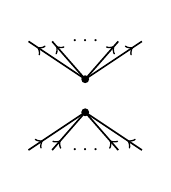
\begin{tikzpicture}[scale=0.6]
    \tikzset{
      lowarrow/.style={semithick,postaction={decorate},
                        decoration={markings, mark=at position 0.25 with {\arrow{>}}}},
      dashedarrow/.style={semithick,postaction={decorate},
                           decoration={markings, mark=at position 0.8 with {\arrow{>}}}},
      outarrow/.style={semithick,postaction={decorate},
                        decoration={markings, mark=at position 0.25 with {\arrow{<}}}}
    }


    \draw[strand,lowarrow] (-1.2,-1.5) -- (0,-0.7);
    \draw[strand,lowarrow] (-0.7,-1.5) -- (0,-0.7);
    
    \node at (0,-1.5) {\scriptsize $\cdots$};

    \draw[strand,lowarrow] (0.7,-1.5) -- (0,-0.7);
    \draw[strand,lowarrow] (1.2,-1.5) -- (0,-0.7);

    \filldraw (0,-0.7) circle (2pt);

    %%%\draw[rdstrand,dashedarrow] (0,-0.7) -- (0,0.0);  %% no det strand for SL

    \filldraw (0,0.0) circle (2pt);

    \draw[strand,outarrow] (-1.2,0.8) -- (0,0.0);
    \draw[strand,outarrow] (-0.7,0.8) -- (0,0.0);

    \node at (0,0.8) {\scriptsize $\cdots$};

    \draw[strand,outarrow] (0.7,0.8) -- (0,0.0);
    \draw[strand,outarrow] (1.2,0.8) -- (0,0.0);
  \end{tikzpicture}}}
}

\newcommand{\Nbox}[1]{
  \vcenter{\hbox{\begin{tikzpicture}[scale=0.6]
  
    \tikzset{lowarrow/.style={semithick, postaction=
                               {decorate},
                               decoration={markings, mark=at position 0.6 with {\arrow{>}}}}}


    \draw[strand,lowarrow] (-1.2,-1.5) -- (-1.2,-0.5);
    \draw[strand,lowarrow] (-0.8,-1.5) -- (-0.8,-0.5);
    \node at (0,-1) {\scriptsize $\cdots$};
    \draw[strand,lowarrow] (0.8,-1.5) -- (0.8,-0.5);
    \draw[strand,lowarrow] (1.2,-1.5) -- (1.2,-0.5);


    \draw[thick,fill=white] (-1.4,-0.5) rectangle (1.4,0.5);
    \node at (0,0) {$#1$};


    \draw[strand,lowarrow] (-1.2,0.5) -- (-1.2,1.5);
    \draw[strand,lowarrow] (-0.8,0.5) -- (-0.8,1.5);
    \node at (0,1) {\scriptsize $\cdots$};
    \draw[strand,lowarrow] (0.8,0.5) -- (0.8,1.5);
    \draw[strand,lowarrow] (1.2,0.5) -- (1.2,1.5);
  \end{tikzpicture}}}
}